\chapter{Procedimiento}
A continuación se describen los procesos del algoritmo que permiten solucionar el problema especificado. El código fuente está disponible de manera digital en la plataforma de GitHub \cite{LindermanDgz}.

\section{Lectura del dataset}
Se comienza leyendo el dataset que contiene información que ha sido etiquetada de manera manual por los autores del mismo. Este proceso se describe en \Cref{code:load_dataset}.

\begin{listing}[!ht]
\inputminted{python}{code_listings/load_dataset.py}
\caption{Cargar las anotaciones del dataset}
\label{code:load_dataset}
\end{listing}

Utilizando la biblioteca \texttt{json} de Python leémos el archivo \texttt{RoCoLE.json} (originalmente \texttt{Annotations/RoCoLE-json.json}). La variable \texttt{annotations} contiene la información necesaria para contruir nuestro conjunto de datos de prueba (véase \Cref{table:required_annotations}).

\begin{table}[h!]
\centering
\begin{tabular}{|l|l|}
\hline 
\textbf{Anotación} & \textbf{Descripción} \\ 
\hline 
ID & Identificador de la hoja \\ 
\hline 
Label.Leaf.0.state & Estado de la hoja como saludable o infectada \\ 
\hline 
Label.classification & Clasificación de la hoja o nivel de afectación \\ 
\hline 
Label.Leaf.0.geometry & Puntos (x,y) que determinan el contorno de la hoja \\ 
\hline 
\end{tabular}
\caption{Anotaciones del dataset}
\label{table:required_annotations}
\end{table}

\subsection{La clase CoffeeLeaf}
A continuación creamos una clase llamada \texttt{CoffeeLeaf} la cual se encarga de contener los datos proporcionados en las anotaciones y que representa a una hoja de café. Los atributos de esta clase pueden observarse en \Cref{code:coffee_leaf}.

\begin{listing}[!ht]
\inputminted{python}{code_listings/coffee_leaf.py}
\caption{La clase CoffeeLeaf}
\label{code:coffee_leaf}
\end{listing}

Una vez creada la clase \texttt{CoffeeLeaf} y leído los datos del dataset, procedemos a crear la lista \texttt{coffee\_leaves} utilizando los datos de la \Cref{table:required_annotations}, tal como se muestra en \Cref{code:coffee_leaves}. El directorio \texttt{../rocole\_photos/} contiene los archivos \texttt{.jepg} del dataset (\texttt{Annotations/RoCoLe-voc.tar.gz/export}).

\begin{listing}[!ht]
\inputminted{python}{code_listings/coffee_leaves.py}
\caption{Lista de objetos CoffeLeaf}
\label{code:coffee_leaves}
\end{listing}

\section{Procesado de la imagen}
Una vez creada la lista \texttt{coffee\_leaves} iniciamos el procesamiento de las imagénes a través de la función \texttt{process} (\Cref{code:process}) de la clase \texttt{CoffeeLeaf}. Véase \Cref{code:process_iteration}.

\begin{listing}[!ht]
\inputminted{python}{code_listings/process.py}
\caption{Función process del la clase CoffeeLeaf}
\label{code:process}
\end{listing}

\begin{listing}[!ht]
\inputminted{python}{code_listings/process_iteration.py}
\caption{Iniciar procesamiento de las imágenes}
\label{code:process_iteration}
\end{listing}

\subsection{Conversión de BGR a RGB}
Debido a que cuando creamos los objetos \texttt{CoffeeLeaf} el argumento \texttt{image\_bgr} pasa datos de una imagen en color \textsf{BGR} (Blue, Green, Red), que es la representación de color por defecto de \textit{OpenCV}, y ya que \textit{matplotlib}, la herramienta para la visualización de las imágenes, utiliza una representación \textsf{RGB} (Red, Green, Blue), una conversión de color es necesaria. Véase \Cref{code:bgr_to_rgb}.

\begin{listing}[!ht]
\inputminted{python}{code_listings/bgr_to_rgb.py}
\caption{Convertir imgen BGR a RGB}
\label{code:bgr_to_rgb}
\end{listing}

El resultado de esta conversión permite visualizar la imagen original (\Cref{img:original}).

\begin{figure}[!ht]
\centering
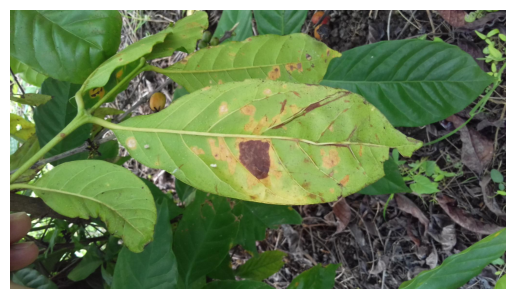
\includegraphics[scale=1]{images/original_image.png}
\caption{Imagen original en RGB}
\label{img:original}
\end{figure}

\subsection{Creación de las regiones de interés}
La anotación \texttt{geometry} del dataset nos provee de una serie de puntos \texttt{(x,y)} que representan el contorno de la hoja de café y que nos sirven para crear un polígono (\Cref{code:polygon}).

\begin{listing}[!ht]
\inputminted{python}{code_listings/polygon.py}
\caption{Puntos (x, y) del contorno de la hoja de café}
\label{code:polygon}
\end{listing}

El contorno de la hoja de café se puede apreciar en la \Cref{img:polygon}.

\begin{figure}[!ht]
\centering
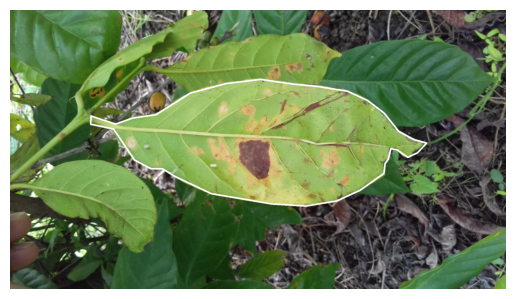
\includegraphics[scale=1]{images/polygon.png}
\caption{Polígono que delimita el contorno de la hoja}
\label{img:polygon}
\end{figure}

Posteriomente creamos el rectángulo mínimo que encierra a esta región, como se aprecia en la \Cref{img:bounding_rect} y lo usamos para recortar nuestra región de interés (véase \Cref{code:roi}).

\begin{figure}[!ht]
\centering
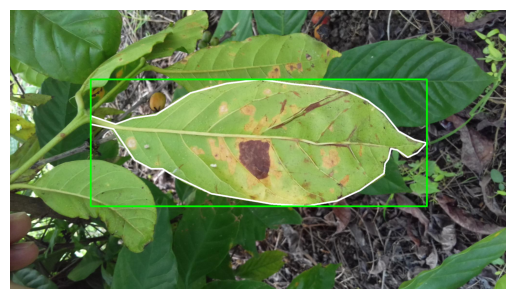
\includegraphics[scale=1]{images/bounding_rect.png}
\caption{Cuadro que aisla a la hoja de café}
\label{img:bounding_rect}
\end{figure}

\begin{listing}[!ht]
\inputminted{python}{code_listings/roi.py}
\caption{Crear regiones de interés}
\label{code:roi}
\end{listing}

Creamos dos regiones de interés: la primera en \textsf{RGB} (\Cref{img:roi_rgb}) para la presentación al usuario y la segunda en \textsf{HSV} (Hue, Saturation, Value) (\Cref{img:roi_hsv}) que nos servirá en la segmentación de la imagen.

\begin{figure}[!ht]
\centering
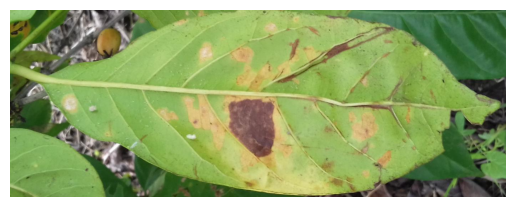
\includegraphics[scale=1]{images/roi_rgb.png}
\caption{Región de interés en RGB}
\label{img:roi_rgb}
\end{figure}

\begin{figure}[!ht]
\centering
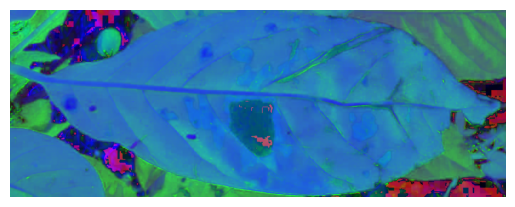
\includegraphics[scale=1]{images/roi_hsv.png}
\caption{Región de interés en HSV}
\label{img:roi_hsv}
\end{figure}

\subsection{Creación de la máscara}
Utilizando las regiones de interés previamente creadas y el polígono que delimita el contorno de la hoja, procedemos a crear una máscara (\Cref{code:mask}) que nos será útil en las operaciones matriciales del procesamiento de la imagen. Véase \Cref{img:mask}.

\begin{listing}[!ht]
\inputminted{python}{code_listings/mask.py}
\caption{Crear máscara}
\label{code:mask}
\end{listing}

\begin{figure}[!ht]
\centering
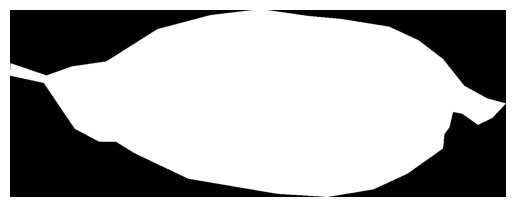
\includegraphics[scale=1]{images/mask.png}
\caption{Máscara}
\label{img:mask}
\end{figure}

Nótese que en \Cref{code:mask} calculamos el área que ocupa la máscara (pixeles en color blanco), o lo que es mismo, el área de la hoja de café.

\subsection{Enmascaramiento de las regiones de interés}
Una vez teniendo la máscara y las regiones de interés, procedemos a \textit{enmascarar} dichas regiones (\Cref{code:masked_roi}). Para el caso de la región de interés en \textsf{RGB} es por mera conveniencia al presentar esta región al usuario. Sin embargo, para el enmascaramiento de la region de interés en \textsf{HSV} es de suma importancia usar únicamente el canal Hue (Matiz) puesto que nuestra segmantación se basará en el color.

\begin{listing}[!ht]
\inputminted{python}{code_listings/masked_roi.py}
\caption{Enmascarar las regiones de interés}
\label{code:masked_roi}
\end{listing}

El resultado de este enmascaramiento se puede apreciar en la \Cref{img:masked_roi_rgb} prara \textsf{RGB} y en la \Cref{img:masked_roi_hue} para \textsf{Hue}.

\begin{figure}[!ht]
\centering
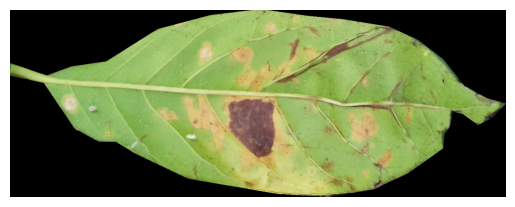
\includegraphics[scale=1]{images/masked_roi_rgb.png}
\caption{Región de interés RGB enmascarada}
\label{img:masked_roi_rgb}
\end{figure}

\begin{figure}[!ht]
\centering
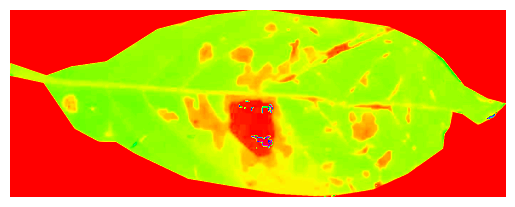
\includegraphics[scale=1]{images/masked_roi_hue.png}
\caption{Región de interés Hue enmascarada}
\label{img:masked_roi_hue}
\end{figure}

Nótese que el valor más bajo para el canal Hue no es un color negro sino un matiz rojo. Esto se debe a la representación circular que emplea el modelo \textsf{HSV}.

\subsection{Histograma de la región de interés}
Una vez que tenemos la región de interés en el canal Hue, procedemos a calcular su histograma (\Cref{code:histogram}) utilizando la máscara (\Cref{img:mask}) de tal manera que no representemos datos fuera del contorno de la hoja. El resultado de la distribución de color puede verse en la \Cref{img:histogram}.

\begin{listing}[!ht]
\inputminted{python}{code_listings/histogram.py}
\caption{Cálcular histograma de la región de interés}
\label{code:histogram}
\end{listing}

\begin{figure}[!ht]
\centering
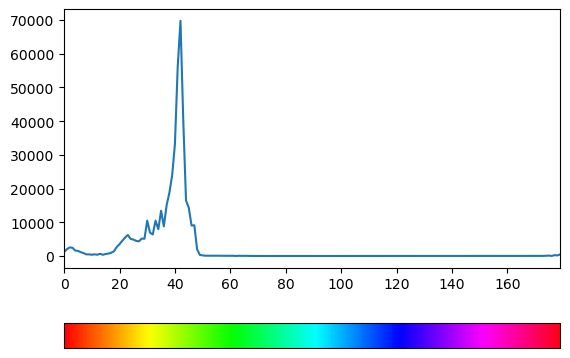
\includegraphics[width=\textwidth]{images/histogram.png}
\caption{Histograma de la región de interés}
\label{img:histogram}
\end{figure}

\subsection{Segmentación de la imagen}
Del histograma nos interesa la región de la hoja que se considera saludable, es decir, la region del espectro Hue en matices verdes, un poco del amarillo-naranja (umbral inferior) y hasta la región azul (umbral superior) para cuando las hojas tengan un verde intenso acercándose a tonos azules.

En el \Cref{code:segmentation} hemos asignado al umbral inferior el valor de 30 y al umbral superior el valor de 120. Segmentamos cada parte de los umbrales y el resultado los unimos usando una operación \texttt{AND} elemento por elemento, resultando en la imagen segmentada apropiadamente (\Cref{img:segmentation}).

\begin{listing}[!ht]
\inputminted{python}{code_listings/segmentation.py}
\caption{Segmentar la región de interés}
\label{code:segmentation}
\end{listing}

\begin{figure}[!ht]
\centering
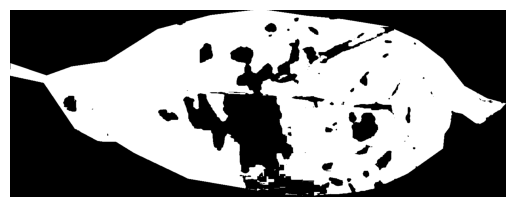
\includegraphics[scale=1]{images/segmentation.png}
\caption{Imagen segmentada}
\label{img:segmentation}
\end{figure}

\subsection{Clasificación de la hoja}
Una vez segmentada la hoja de café en su parte saludable (pixeles blancos) e infectada (pixeles negros dentro de la máscara), procedemos a clasificarla utilizando la misma ponderación usada por los autores (REF Tabla).

Para el cálculo del porcentaje afectado, simplemente calculamos el área saludable de la hoja a partir de la imagen segmentada (\Cref{img:segmentation}) y restamos este valor al área de la máscara (\Cref{code:mask}), como se describe en \Cref{code:categorize}.

\begin{listing}[!ht]
\inputminted{python}{code_listings/categorize.py}
\caption{Clasificar hoja de café}
\label{code:categorize}
\end{listing}

Esta clasificación marca el fin del algoritmo para el procesamiento de la imagen, obteniéndose dos categorías: 1) el estado de la hoja y 2) el nivel de afectación en caso de ser una hoja infectada.

\section{Presentación de los datos}

\subsection{Resumen}
\begin{listing}[!ht]
\inputminted{python}{code_listings/show_summary.py}
\caption{Mostrar resumen de la clasificación}
\label{code:show_summary}
\end{listing}

\subsection{Imagen original}
\begin{listing}[!ht]
\inputminted{python}{code_listings/show_original_image.py}
\caption{Mostrar imagen original}
\label{code:show_original_image}
\end{listing}

\subsection{Máscara}
\begin{listing}[!ht]
\inputminted{python}{code_listings/show_mask.py}
\caption{Mostrar máscara}
\label{code:show_mask}
\end{listing}

\subsection{Regiones de interés}
\begin{listing}[!ht]
\inputminted{python}{code_listings/show_roi.py}
\caption{Mostrar regiones de interés}
\label{code:show_roi}
\end{listing}

\subsection{Imagen segmentada}
\begin{listing}[!ht]
\inputminted{python}{code_listings/show_segmentation.py}
\caption{Mostrar segmentación de la imagen}
\label{code:show_segmentation}
\end{listing}

\subsection{Histograma}
\begin{listing}[!ht]
\inputminted{python}{code_listings/show_histogram.py}
\caption{Mostrar histograma de la región de interés}
\label{code:show_histogram}
\end{listing}